
\section{Software Engineering}

\subsection{Introduction}

\begin{frame}
\frametitle{Software Engineering}
A core challenge for bringing autonomous driving to market is the sheer scale
of the engineering effort required.
\begin{itemize}
    \item Software must be developed that will scale in terms of complexity
        and the number of developers working on it
    \item Integration, testing and deployment must be efficient, fast and
        reliable
    \item A large number of engineers must be coordinated to work towards a
        single, common goal
    \item Product and development process must comply to a wide range of
        industry standards
\end{itemize}
\pause
\begin{block}{}
These aspects of software engineering are often the majority of the effort 
required for developing a product $\rightarrow$ the functional application
may be simple in comparison.
\end{block}
\end{frame}

\begin{frame}
\frametitle{Software Best Practices}
It is important that the code you write can be easily understood by someone
you may never meet, several years later, long after you've left the project
or company.

\begin{columns}[]
    \begin{column}{0.65\textwidth}
        \begin{itemize}
            \item Practice clean code
            \begin{itemize}
                \item Use human-understandable and meaningful variable/function/class
                    names
                \item Keep method/function size small
                \item The code \emph{is} the documentation
            \end{itemize}
            \item Follow the SOLID and DRY principles
            \item Minimize technical debt
            \item Code reviews are a must
            \item Use coding guidelines and enforce them with linters
        \end{itemize}   
    \end{column}
    \begin{column}{0.35\textwidth}
        \centering
        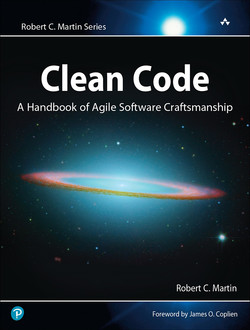
\includegraphics[height=0.75\textwidth]{images/book_clean_code.jpg}\\
        \footnotesize{\emph{Clean Code} by Robert C. Martin\footnotemark[1]}
    \end{column}
\end{columns}
\footnotetext[1]{\tiny{\url{https://www.oreilly.com/library/view/clean-code-a/9780136083238/}}}
\end{frame}

% \begin{frame}
% \frametitle{Software Best Practices}
% The SOLID principles, introduced by Robert C. Martin, are a great guide
% for designing software that is understandable and maintainable.
% \begin{itemize}
%     \item \textbf{S}ingle-Responsibility Principle: Function/classes/etc.
%         should do only \emph{one} thing.
%     \item \textbf{O}pen-Closed Principle: Entities are open for extension, but
%         closed for modification. 
%     \item \textbf{L}iskov Substitution Principle: If S is a subtype of T, then
%         objects of type T may be replaced with objects of type S
%     \item \textbf{I}nterface Segregation Principle: 
%     \item \textbf{D}ependency Inversion Principle:
% \end{itemize}
% The SOLID principles can also be applied to functional and software
% architecture and design. The Clean Architecture\footnotemark[1] book is a great
% reference.
% \footnotetext[1]{\tiny{\url{https://www.oreilly.com/library/view/clean-architecture-a/9780134494272/}}}
% \end{frame}

\subsection{CI/CD}

\begin{frame}
\frametitle{Continuous Integration / Delivery / Deployment}
Modern software engineering is not feasible without continuous integration and
continuous deployment.\\

\textbf{Continuous Integration}: Automated building, testing, and integration 
with every change in the software.\\

\textbf{Continuous Delivery}: Release artifacts are created and automatically
tested in pre-production environments. Deployment into the field is done
manually.\\

\textbf{Continuous Deployment}: Ability to deploy software into the field
automatically.\\

\pause

\begin{block}{}
What does CI/CD looks like in practice for an autonomous vehicles?
\end{block}
\end{frame}

\begin{frame}
\frametitle{Continuous Integration / Deployment}
\framesubtitle{Pipeline for a fleet of autonomous vehicles}
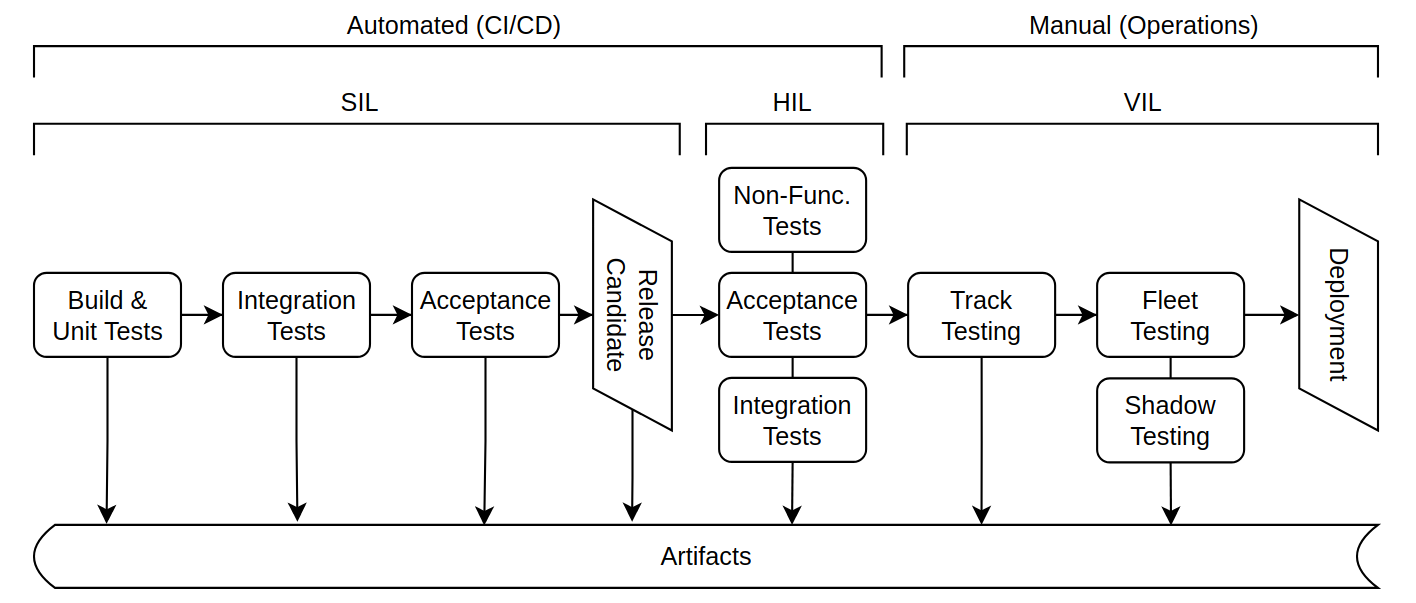
\includegraphics[width=\textwidth]{images/autonomous_driving_ci-cd_pipeline.png}
\end{frame}

\begin{frame}
\frametitle{Continuous Integration / Deployment}
\framesubtitle{Example CI/CD pipeline from Apex.AI}
\centering
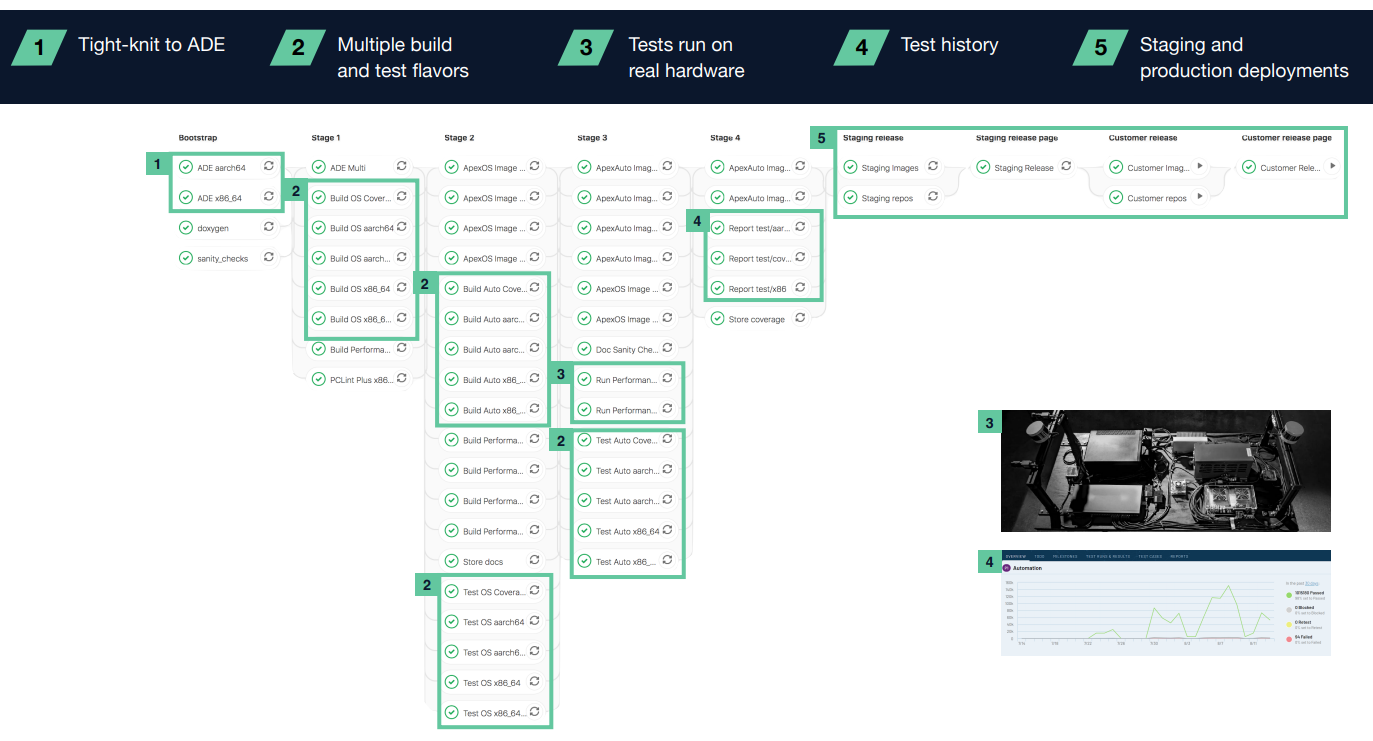
\includegraphics[height=0.78\textheight]{images/apex_cicd.png}\\
\footnotesize{Source: Apex.AI}
\end{frame}

\subsection{Testing}

\begin{frame}
\frametitle{Testing}
Software testing is a vital aspect of successful software development, in
particular for a safety-relevant application such as autonomous vehicles.

\begin{itemize}
    \item Treat test code to the same standards as production code
    \item The amount of test code will likely be multiple factors larger 
        than the actual production application code
    \item Tests should be automated, repeatable and independent
    \item Test the behavior, not the implementation
    \item Follow Arrange - Act - Assert pattern
    \item The scope of the system under test should be increased with every
        stage of a CI/CD pipeline
\end{itemize}
\end{frame}

\begin{frame}[fragile]
\frametitle{Unit Testing}
Testing of the smallest, simplest entities, e.g. classes, functions, etc.\\
\begin{columns}[]
    \begin{column}{0.5\textwidth}
        \begin{itemize}
            \item Tests are lightning fast
            \item Number of tests is incredibly large
            \item Tests have no external dependencies (e.g. to file system, etc.)
            \item Test expected failure cases, e.g. invalid input
            \item GoogleTest\footnotemark[1] for C++
        \end{itemize}
    \end{column}
    \begin{column}{0.5\textwidth}
\tiny
\begin{minted}{cpp}
TEST(VehicleSpeedChecks, IsVehicleOverSpeedLimit)
{
    // Arrange
    constexpr float vehicle_speed_kmh = 120;
    constexpr float speed_limit_kmh = 100;

    // Act
    auto speeding =
        isVehicleSpeeding(vehicle_speed_kmh, speed_limit_kmh);

    // Assert
    EXPECT_TRUE(speeding);
}
\end{minted}
    \end{column}
\end{columns}
\begin{exampleblock}{Example for autonomous vehicles}
Individual functions from a Kalman filter library, e.g. predict(), are tested.
\end{exampleblock}
\footnotetext[1]{\tiny{\url{https://github.com/google/googletest}}}
\end{frame}

\begin{frame}
\frametitle{Integration Testing}
Multiple components of a system are tested together.
\begin{itemize}
    \item Black-box testing (implementation details of components are not known)
    \item Tests interfaces and interactions between components
    \item Input is more complex
    \item Tests may run longer and take more resources
    \item May interact with external dependencies, e.g. file system
    \item In ROS, the launch\_testing\footnotemark[1] framework can be used to
        do integration testing on a system of nodes
\end{itemize}
\begin{exampleblock}{Example for autonomous vehicles}
A lidar perception pipeline is tested, e.g. the components of clustering and
tracking are tested together.
\end{exampleblock}
\footnotetext[1]{\tiny{\url{https://github.com/ros2/launch/tree/master/launch_testing}}}
\end{frame}

\begin{frame}
\frametitle{Acceptance Testing}
Testing the overall product behavior based on functional and business
requirements.
\begin{itemize}
    \item Validates the product requirements
    \item Requires interaction between product/business and engineering
    \item Simulations or recorded data can be used as input
    \item Given - When - Then pattern
    \item Cucumber\footnotemark[1] framework
    \item Often called \emph{Scenario-based Testing} in the autonomous vehicles
        space
\end{itemize}
\begin{center}
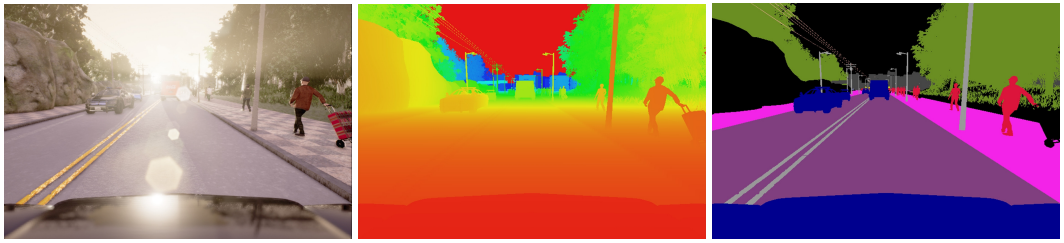
\includegraphics[width=0.42\textwidth]{images/carla_simulation.png}\\
\footnotesize{CARLA open source simulator for autonomous driving \cite{Dosovitskiy17}}
\end{center}
\begin{exampleblock}{Example for autonomous vehicles}
The vehicle behaves correctly when approaching a red light.
\end{exampleblock}
\footnotetext[1]{\tiny{\url{https://cucumber.io/}}}
\end{frame}

\begin{frame}
\frametitle{Manual Acceptance Testing}
\begin{columns}[]
    \begin{column}{0.55\textwidth}
        Some acceptance testing is impossible, or very difficult, to automate,
        which still requires some testing to be done manually.\\
        \begin{itemize}
            \item Interaction with users is required, e.g. user acceptance testing
            \item System under test is increased to include artifacts of the
                physical, which cannot be automated in computer systems
        \end{itemize}
    \end{column}
    \begin{column}{0.45\textwidth}
        \centering
        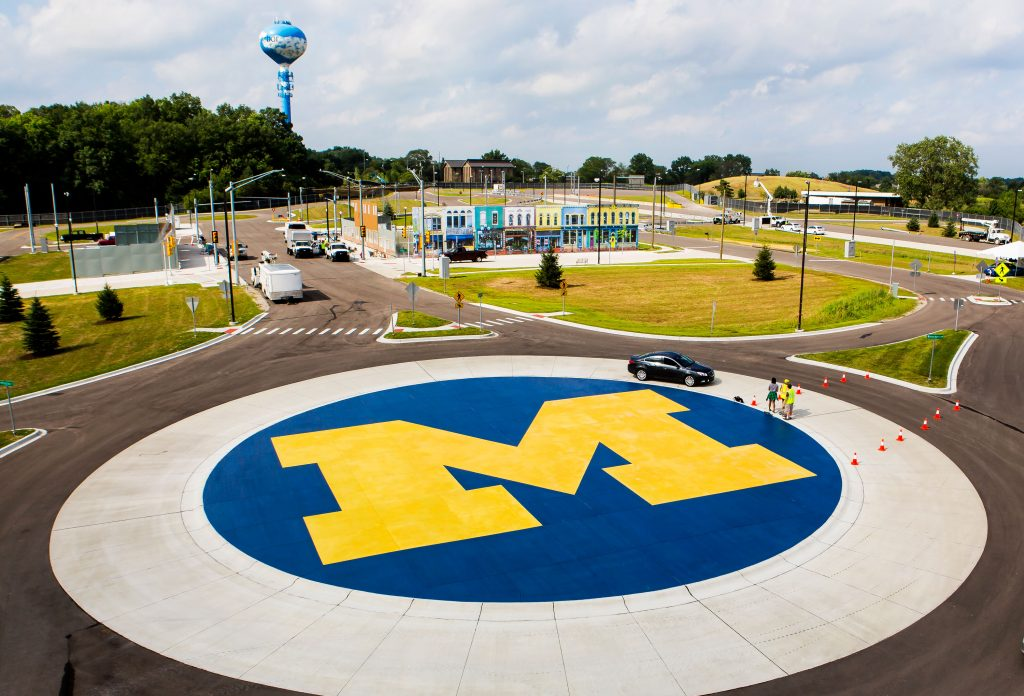
\includegraphics[width=0.8\textwidth]{images/m-city.jpg}\\
        \footnotesize{Mcity Test Facility at University of Michigan\footnotemark[1]}
    \end{column}
\end{columns}
\begin{exampleblock}{Example for autonomous vehicles}
In-vehicle testing with a safety-driver, either on the test track or with a
fleet on public roads.
\end{exampleblock}
\footnotetext[1]{\tiny{\url{https://mcity.umich.edu/our-work/mcity-test-facility/}}}
\end{frame}

\begin{frame}
\frametitle{Test-Driven Development}
Methodology for ensuring all written code is thoroughly tested.
\begin{columns}[]
    \begin{column}{0.6\textwidth}
        \begin{itemize}
            \item Tests are written first!
            \item Forces developer to think about the behavior of the code
                they are about to write
            \item Improved API design, since tests are written from the
                perspective of the user
            \item Leads to improved software architecture with reduced
                dependencies
            \item CI can be utilized from the beginning to protect the code
        \end{itemize}
    \end{column}
    \begin{column}{0.4\textwidth}
        \centering
        \smartdiagramset{
            module minimum width=2cm,
            module minimum height=1cm,
            text width=2cm,
            circular distance=2cm,
            set color list={red!40,green!40,blue!40}
        }
        \smartdiagram[circular diagram:clockwise]{
            Write a failing test,
            Make the test pass,
            Refactor
        }
    \end{column}
\end{columns}
\end{frame}

\subsection{Development Process}

\begin{frame}
\frametitle{Development Process}
\framesubtitle{An overview}
It is inevitable that once a project becomes larger than a few core developers,
a development process will emerge such that everyone involved is able move
towards a common goal and "speak the same language".\\

A development process divides the work into separate steps or processes which
are to be followed and which have defined artifacts, outcomes, expectations,
etc.\\

Let's review three common development processes in the automotive industry:
\begin{itemize}
    \item Waterfall
    \item V-Model
    \item Agile
\end{itemize}
\end{frame}

\begin{frame}
\frametitle{Waterfall}
The waterfall approach is the most extreme interpretation of an ideal
development process, where each phase of development follows a strict
linear progression.
\begin{columns}[]
    \begin{column}{0.5\textwidth}
        \begin{itemize}
            \item Assumes that requirements, architecture design, etc. are
                correct and fully known before development begins
            \item Testing is the last step in the process where major issues
                could be uncovered
            \item The automotive industry, as a traditional mechanical
                engineering discipline, has had a tendency to apply this
                methodology, despite its pitfalls
        \end{itemize}
    \end{column}
    \begin{column}{0.5\textwidth}
        \centering
        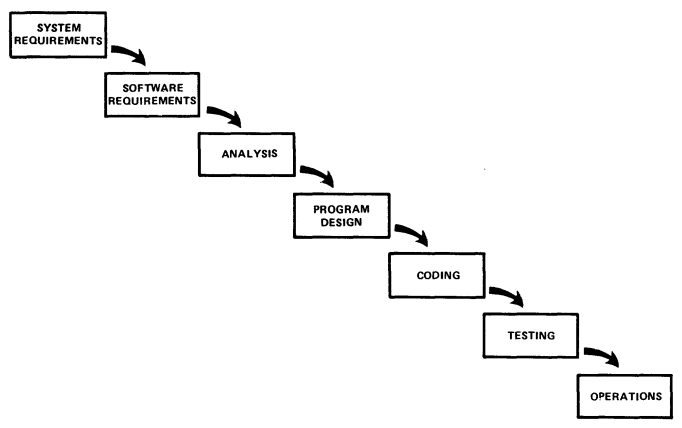
\includegraphics[width=0.8\textwidth]{images/royce_waterfall.png}\\
        \footnotesize
        First figure of Royce's 1970 paper \cite{Royce70} (which is not what
        the paper proposes)
    \end{column}
\end{columns}
\end{frame}

\begin{frame}
\frametitle{V-Model}
The V-Model development process has been the mainstream process in the
automotive industry, in particular in Germany. The process is often mandated
by standards, contract obligations, etc.
\begin{columns}[]
    \begin{column}{0.6\textwidth}
        \begin{itemize}
            \item Originally developed in the defense industry
            \item Validation and Verification must prove the requirements and
                design
            \item Often interpreted and therefore implemented with a time
                axis at the bottom of the V
        \end{itemize}
    \end{column}
    \begin{column}{0.4\textwidth}
        \centering
        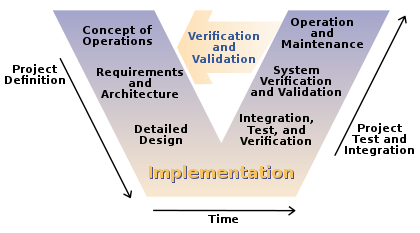
\includegraphics[width=0.9\textwidth]{images/v-model.png}\\
        \footnotesize Source: Wikipedia\footnotemark[1]
    \end{column}
\end{columns}
\begin{block}{}
Similar issues as in the waterfall process may raise: project definition
assumptions and design may be invalidated during testing and risk that the
project does not deliver on time.
\end{block}
\footnotetext[1]{\tiny{\url{https://en.wikipedia.org/wiki/V-Model}}}
\end{frame}

\begin{frame}
\frametitle{Agile}
In 2001, several a group of software developers formulated their frustrations
with current state of software development, and came up with the
\emph{Agile Manifesto}\footnotemark[1].
\vspace{0.25cm}
\begin{itemize}
    \item \textbf{Individuals and interactions} over processes and tools
    \item \textbf{Working software} over comprehensive documentation
    \item \textbf{Customer collaboration} over contract negotiation
    \item \textbf{Responding to change} over following a plan
\end{itemize}
\vspace{0.25cm}
The 12 principles they formulated form the basis of agile and the many related
methodologies and processes that are practiced today.
\footnotetext[1]{\tiny{\url{https://agilemanifesto.org/}}}
\end{frame}

\begin{frame}
\frametitle{Scrum}
A development process designed with the agile manifesto in mind, created by 
one of its authors, Jeff Sutherland.
\begin{columns}[]
    \begin{column}{0.5\textwidth}
        \begin{itemize}
            \item Short iterations (2-4 weeks) of focused and committed
                development to finish new features
            \item Work is visible and prioritized via the product backlog
            \item Well-defined roles and "rituals" within a Scrum team
        \end{itemize}
    \end{column}
    \begin{column}{0.5\textwidth}
        \centering
        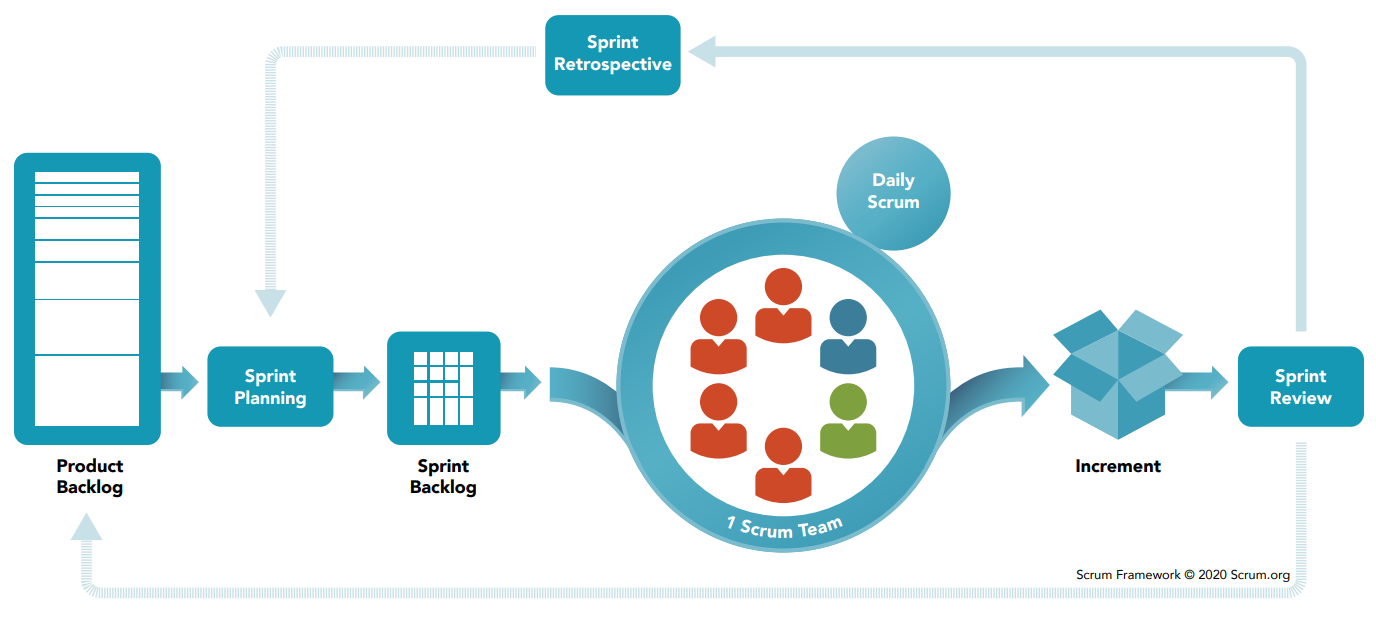
\includegraphics[width=\textwidth]{images/scrum.png}\\
        \footnotesize Source: Scrum.org\footnotemark[1]
    \end{column}
\end{columns}
\begin{block}{}
This work great for one team, but what if you have an organization of hundreds,
or thousands of developers?
\end{block}
\footnotetext[1]{\tiny{\url{https://www.scrum.org/}}}
\end{frame}

\begin{frame}
\frametitle{SAFe - Scaled Agile Framework}
\centering
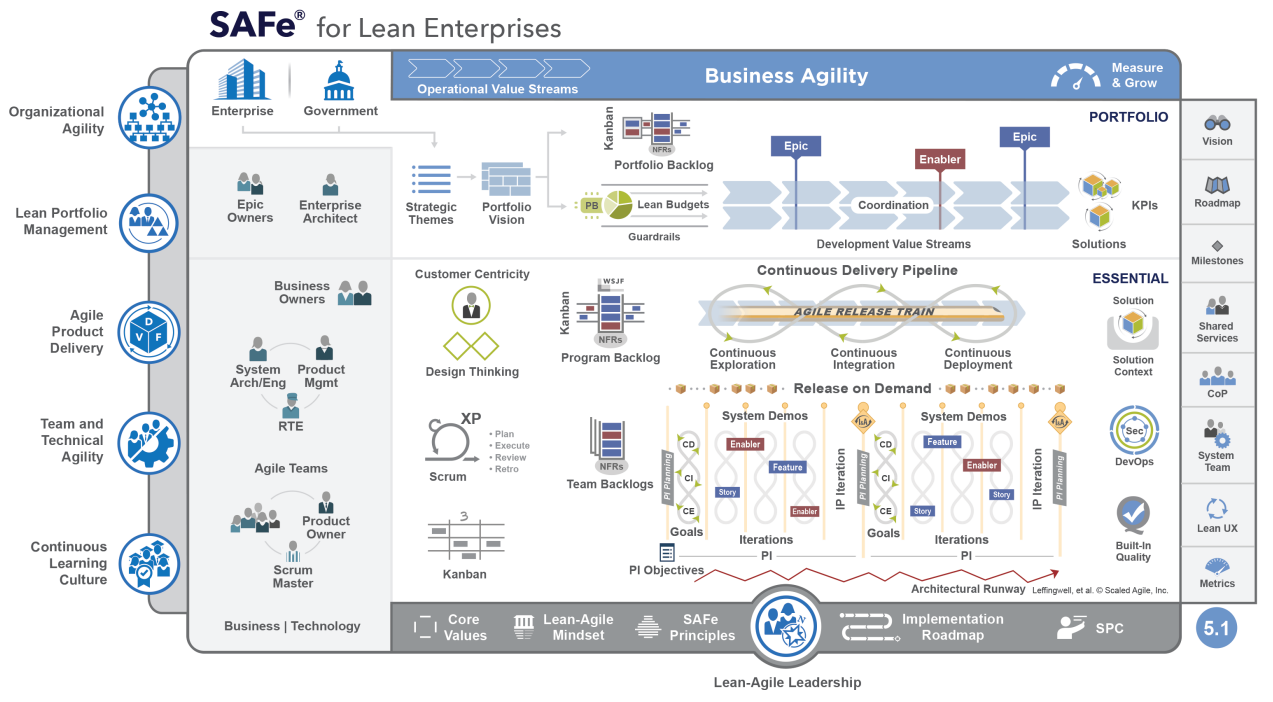
\includegraphics[width=0.8\textwidth]{images/agile-safe.png}\\
\footnotesize Source: Scaled Agile Framework\footnotemark[1]
\footnotetext[1]{\tiny{\url{https://www.scaledagileframework.com/}}}
\end{frame}

\begin{frame}
\frametitle{LeSS - Large-Scale Scrum}
\begin{center}
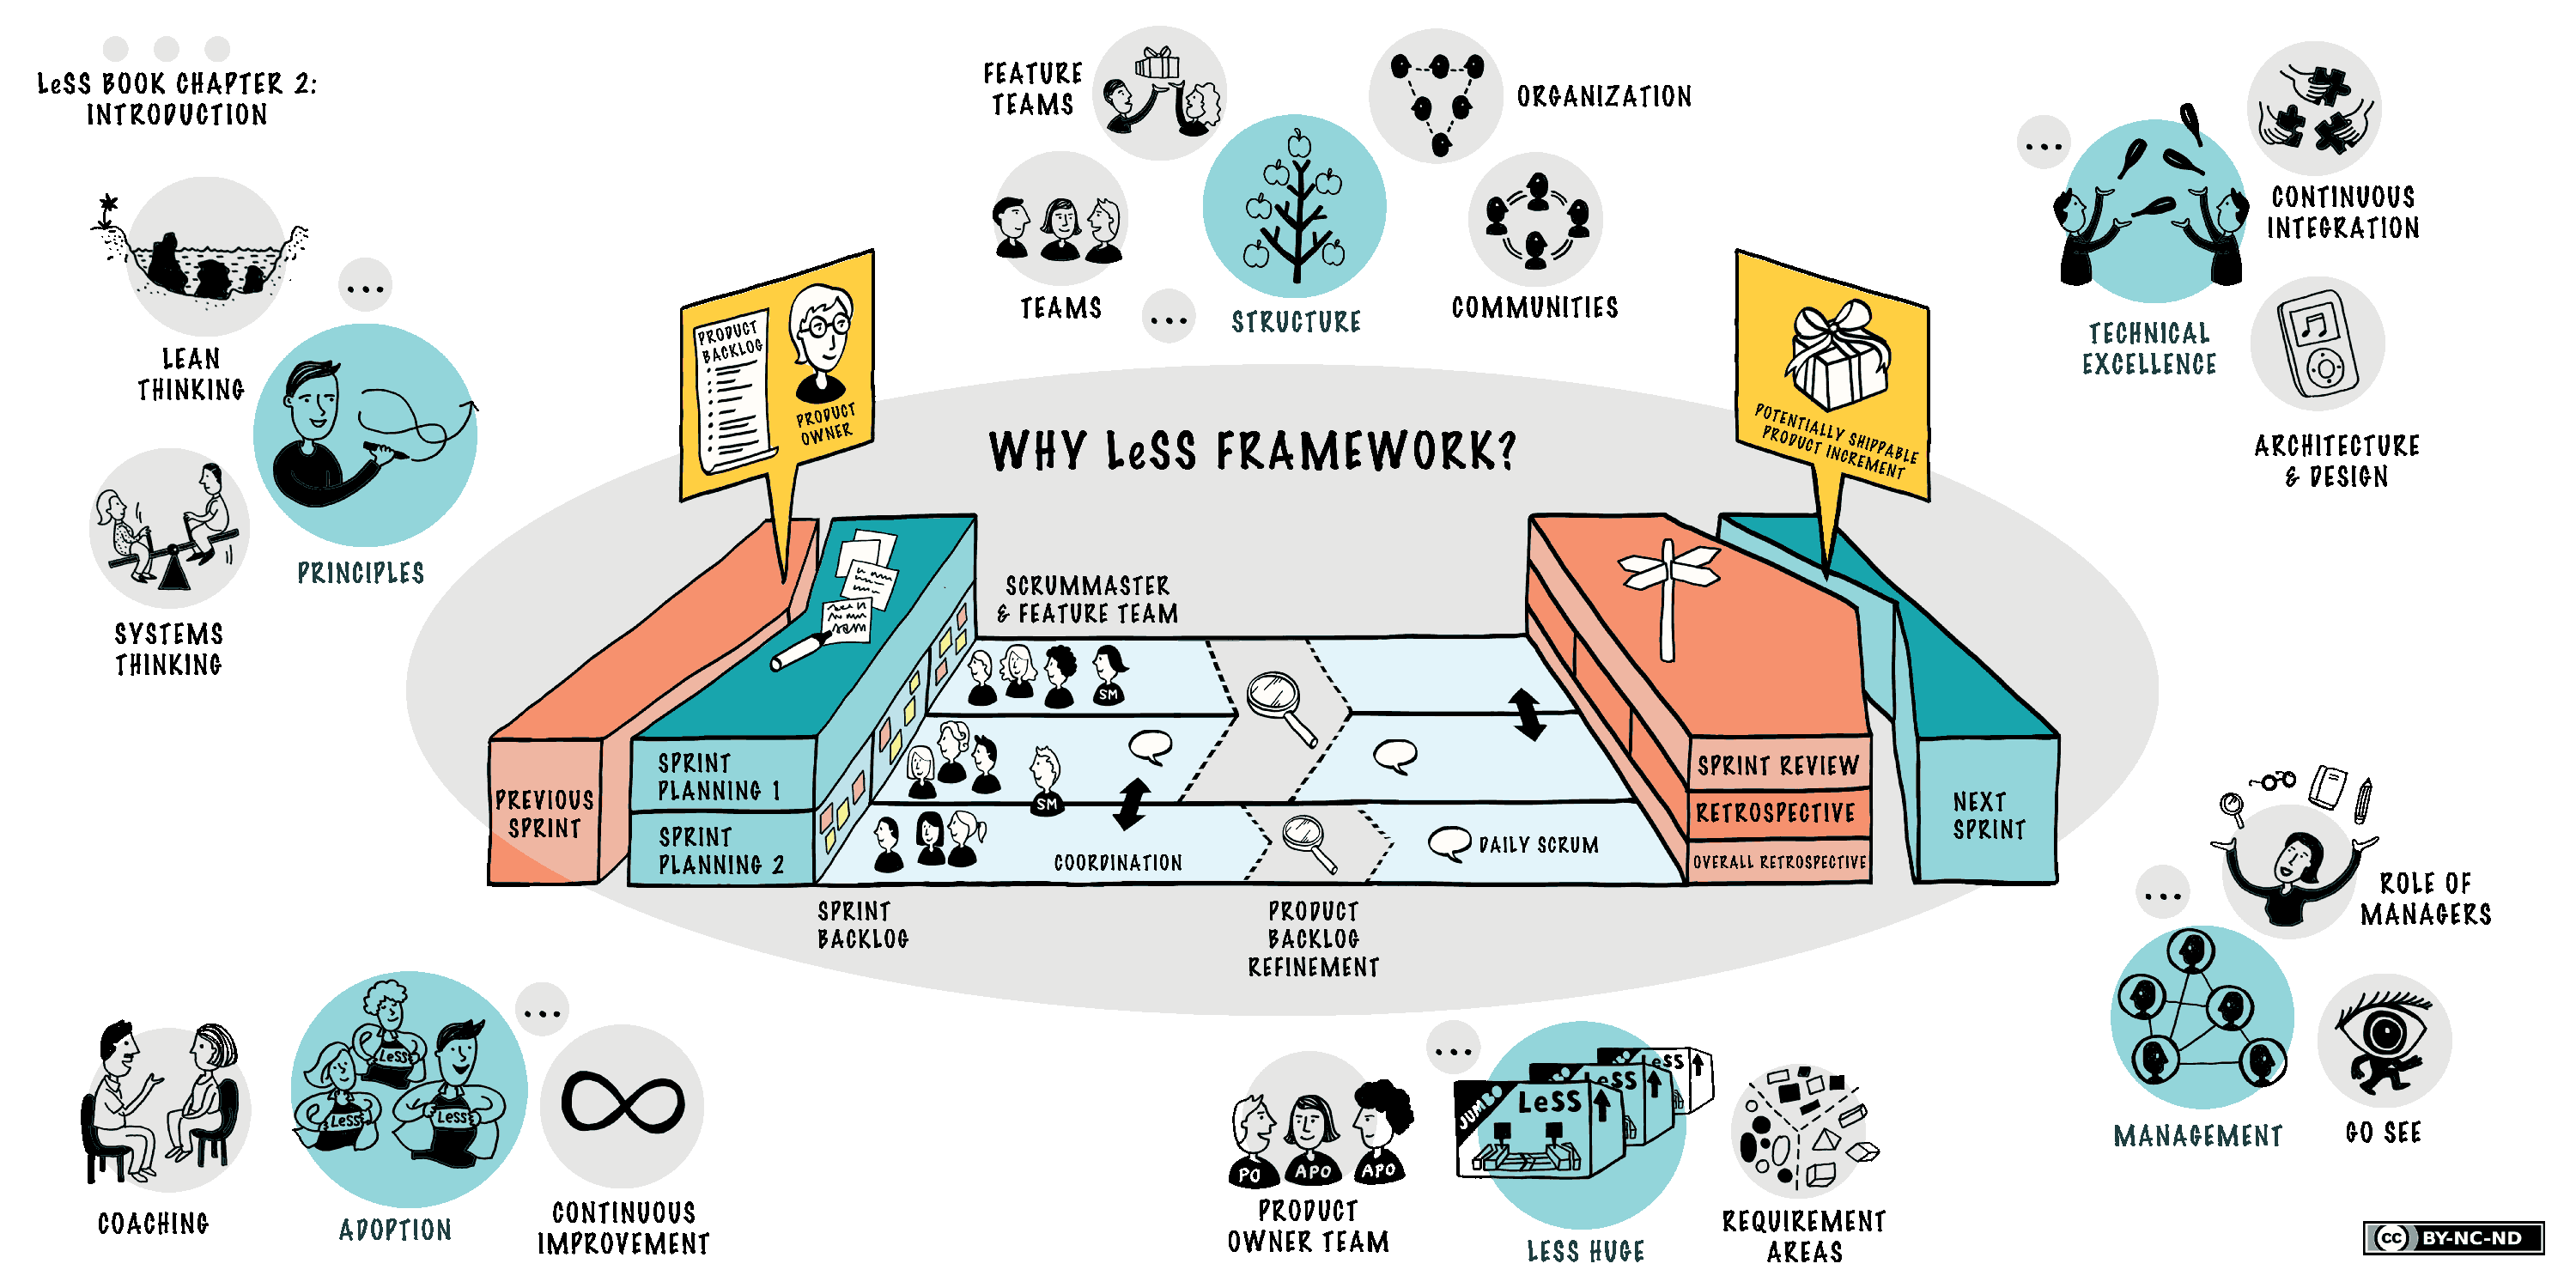
\includegraphics[width=0.6\textwidth]{images/agile-less.png}\\
\footnotesize Source: Large-Scale Scrum (LeSS)\footnotemark[1]\\
\end{center}
LeSS Huge was adopted by BMW Group's Autonomous Driving division.\footnotemark[2] 
\footnotetext[1]{\tiny{\url{https://less.works/}}}
\footnotetext[2]{\tiny{\url{https://less.works/case-studies/bmw-group-autonomous-driving}}}
\end{frame}

\begin{frame}
\frametitle{Agile}
\framesubtitle{Some thoughts...}
Despite the craze/hype with agile in today's software engineering industry, one
should step back and reflect...\\
\begin{itemize}
    \item Not everything has to be black-and-white and follow a known process
        $\rightarrow$ each company (and its people) and product are different,
        so do what works for you
    \item Most development processes have the same intention: deliver
        high-quality, well-tested, and on-time software that bring value to the
        customer
    \item Often the same technical development practices are encouraged
        $\rightarrow$ best to get those right
    \item Don't forget the V-Model $\rightarrow$ why not combine it with agile?
\end{itemize}
\end{frame}

\subsection{Standards}

\begin{frame}
\frametitle{Standards}
Developing a commercial product, in particular a safety-critical product such
as autonomous driving, requires the compliance to industry best-practices,
often defined by industry standards and guidelines.\\

The automotive industry is no exception, where many standards influence the
daily work of a software developer.
\end{frame}

\begin{frame}
\frametitle{ASPICE}
\begin{columns}[T]
    \begin{column}{0.4\textwidth}
        Defines a software development process to be followed in the automotive
        industry.\\
        \begin{itemize}
            \item Based on the V-Model
            \item OEMs often require compliance for their suppliers
            \item Applies also to non-safety software
            \item Defines non-technical work, such as supplier contracting
        \end{itemize}
    \end{column}
    \begin{column}{0.6\textwidth}
        \centering
        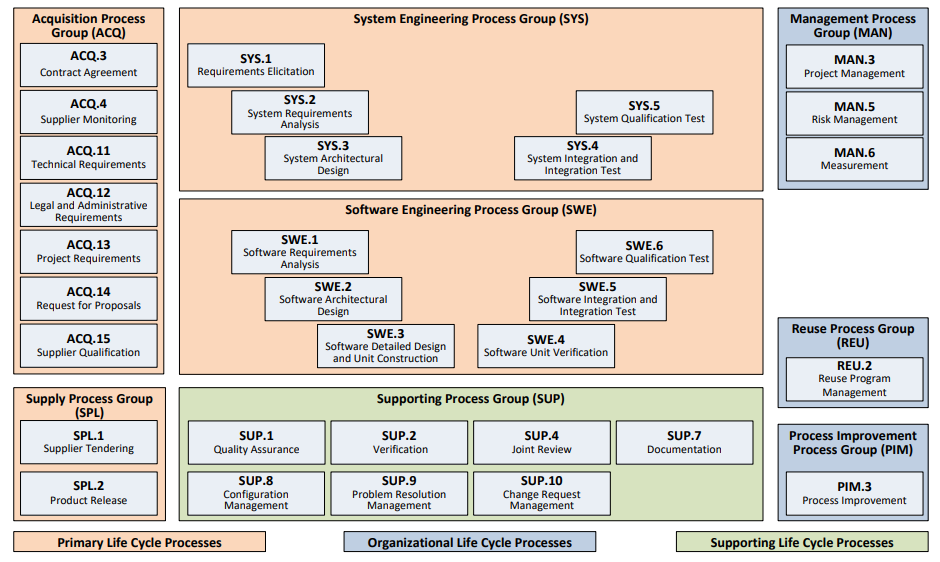
\includegraphics[width=\textwidth]{images/aspice.png}\\
        \footnotesize Source: Automotive SPICE$^{\tiny{\textregistered}}$
            Process Reference and Assessment Model\footnotemark[1]
    \end{column}
\end{columns}
\footnotetext[1]{\tiny{\url{https://automotivespice.com/}}}
\end{frame}

\begin{frame}
\frametitle{Standards for Safety}
\framesubtitle{ISO 26262 - Functional Safety for Road Vehicles}
\begin{columns}[]
    \begin{column}{0.6\textwidth}
        ISO 26262 defines a development standard and practices for functional safety
        applications implemented in hardware (electrical) and software.\\
        \begin{itemize}
            \item Designed to protect against faults in E/E system
            \item Analysis of a system from a safety perspective
            \item Derive risks, safety goals, safety mechanisms
            \item Safety integrity levels (ASIL) are defined, which impose
                requirements on the process and implementation
            \item Example result: monitoring mechanisms, testing,
                system redundancy, etc.
        \end{itemize}
    \end{column}
    \begin{column}{0.4\textwidth}
        \centering
        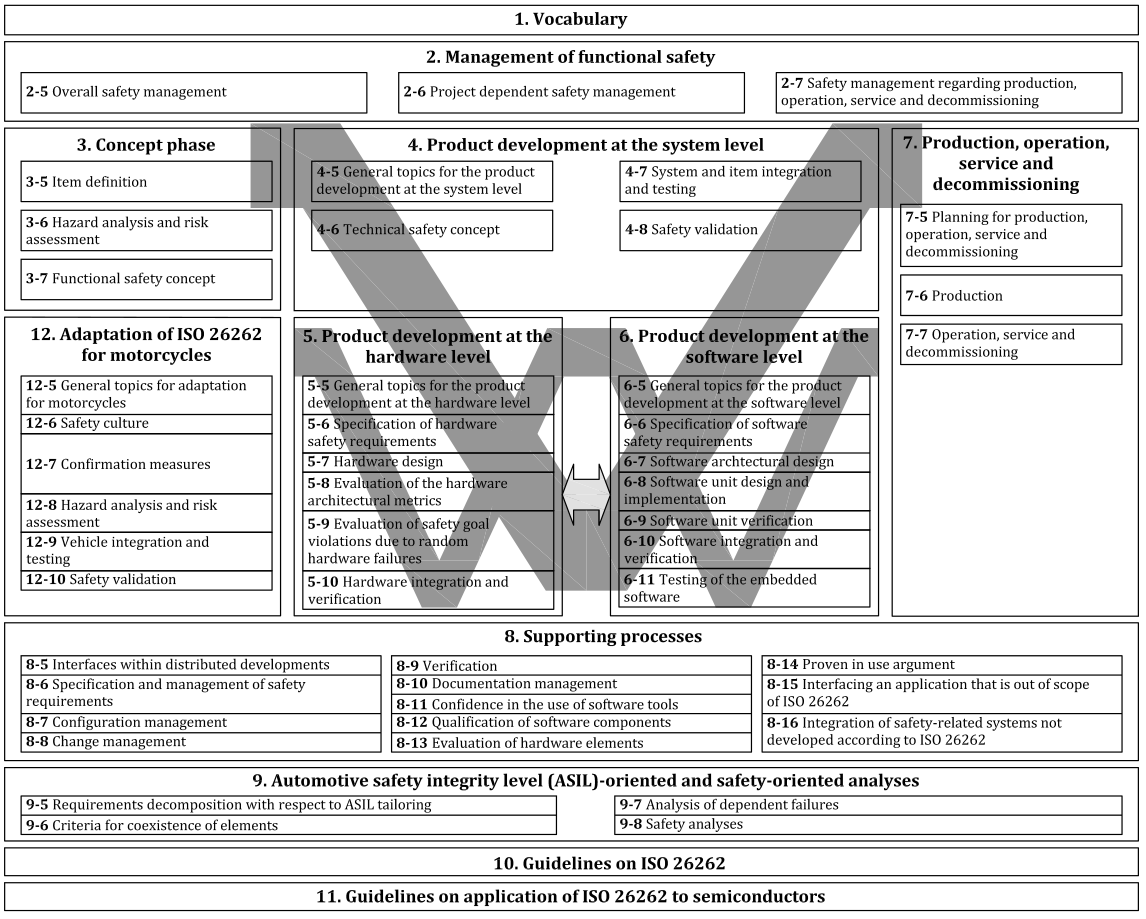
\includegraphics[width=\textwidth]{images/iso26262.png}\\
        \footnotesize Source: ISO 26262-1:2018 \cite{ISO26262}
    \end{column}
\end{columns}
\end{frame}

\begin{frame}
\frametitle{Standards for Safety}
\framesubtitle{ISO 21448 - Safety of the Intended Functionality (SOTIF)}
\begin{columns}[]
    \begin{column}{0.65\textwidth}
        Supplemental standard to ISO 26262 designed to protect against
        performance limitations of the system or intentional misuse.
        \begin{itemize}
            \item Definition of use-cases and scenarios to guide the development
                of relevant testing procedures
            \item Goal is to reduce the space of known/unknown unsafe scenarios
            \item Proposes methods for verification of SOTIF
            \item Annex B shows an example for mitigating
                false alarm rate in AEB systems
            \item Example result: scenarios for acceptance testing (automated
                and manual) are defined, found, and verified
        \end{itemize}
    \end{column}
    \begin{column}{0.35\textwidth}
        \centering
        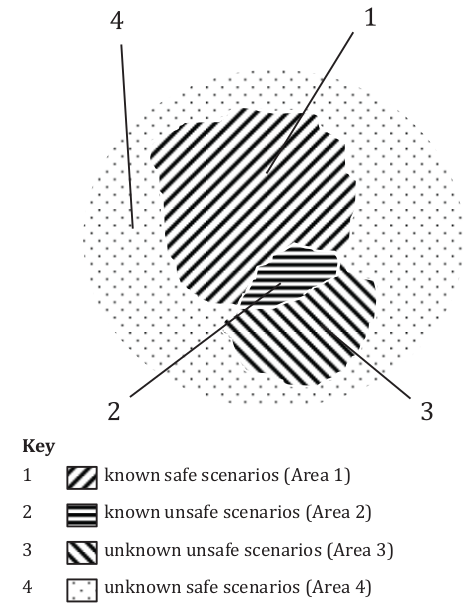
\includegraphics[width=0.80\textwidth]{images/sotif_scenarios.png}\\
        \footnotesize Source: ISO/PAS 21448:2019 \cite{ISO21448}
    \end{column}
\end{columns}
\end{frame}

% \begin{frame}
% \frametitle{Security}
% \end{frame}

\begin{frame}
\frametitle{Coding Guidelines}
Coding guidelines are used to impose restrictions on programming languages such
that common errors or language misuse risks are mitigated.\\
\begin{columns}[]
    \begin{column}{0.5\textwidth}
        \begin{itemize}
            \item Static analysis tools like axivion\footnotemark[1] are available
                to automatically validate code against such guidelines
            \item AUTOSAR C++ 14 \cite{AutosarCpp14} and MISRA C++ \cite{MisraCpp} are
                common guidelines used for the C++ language
        \end{itemize} 
    \end{column}
    \begin{column}{0.5\textwidth}
        \emph{Examples from AUTOSAR C++ 14 \cite{AutosarCpp14}:}\\
        \vspace{0.25cm}
        \footnotesize
        \textbf{Rule M0-1-3}: A project shall not contain unused variables.\\
        \vspace{0.1cm}
        \textbf{Rule A12-6-1}: All class data members that are initialized by the
        constructor shall be initialized using member initializers.\\
        \vspace{0.1cm}
        \textbf{Rule A18-0-2}: The library functions atof, atoi and atol from
        library <cstdlib> shall not be used.\\
        \vspace{0.1cm}
        \textbf{Rule A18-5-2}: Operators new and delete shall not be called
        explicitly.\\
    \end{column}
\end{columns}
\footnotetext[1]{\tiny{\url{https://www.axivion.com/en/products/coding-guidelines/autosar-c14-check/}}}
\end{frame}

\begin{frame}
\frametitle{Autonomous Vehicle Ecosystem Landscape}
\begin{columns}[]
    \begin{column}{0.4\textwidth}
        \centering
        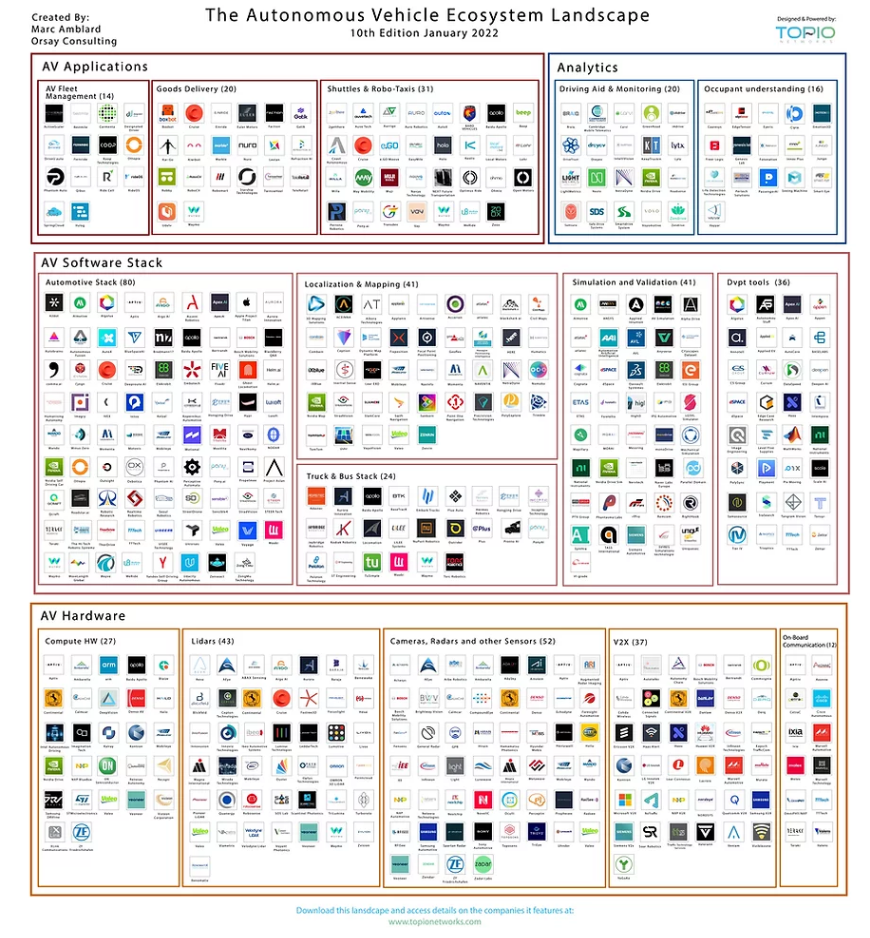
\includegraphics[height=0.75\textheight]{images/av_ecosystem_landscape.png}\\
        \footnotesize{Source: Orsay Consulting\footnotemark[1]}        
    \end{column}
    \begin{column}{0.6\textwidth}
        Autonomous vehicles and software engineering are taking over the
        automotive industry.
        \begin{itemize}
            \item Many companies, big and small, are providing solutions across
                the whole stack
            \item In-vehicle, cloud, and supporting infrastructure software
                need to seamlessly work together
            \item Efficient development tools are required
        \end{itemize}
        \begin{block}{}
        Many opportunities for aspiring software engineers!
        \end{block}
    \end{column}
\end{columns}
\footnotetext[1]{\tiny{\url{https://www.orsayconsulting.net/mobility-resources-en}}}
\end{frame}